% GENIE5 - CS491 Project Specification Report (short version)
% Structure follows the course guideline. Compile with pdfLaTeX (Overleaf), two passes.
% The detailed design, the experiments and the ideas we do not commit to are in
% docs/design-notes.tex. This report states only what is built or planned with confidence.

\documentclass[11pt,a4paper]{article}

\usepackage[utf8]{inputenc}
\usepackage[T1]{fontenc}
\usepackage[margin=2.5cm]{geometry}
\usepackage{lmodern}
\usepackage{microtype}
\usepackage{booktabs}
\usepackage{tabularx}
\usepackage{longtable}
\usepackage{enumitem}
\usepackage{xcolor}
\usepackage{float}
\usepackage{needspace}
\usepackage{tikz}
\usepackage{pgfplots}
\pgfplotsset{compat=1.18}
\usetikzlibrary{arrows.meta, fit, backgrounds}
\usepackage{hyperref}
\usepackage{xurl}

\hypersetup{colorlinks=true, linkcolor=black, urlcolor=blue!50!black, citecolor=black}
\setlength{\parskip}{0.5em}
\setlength{\parindent}{0pt}
\setlist{itemsep=0.15em, topsep=0.3em}
\renewcommand{\arraystretch}{1.25}

\newcommand{\gen}{GENIE5}
\newcommand{\code}[1]{\texttt{#1}}
\newcolumntype{L}{>{\raggedright\arraybackslash}X}

\begin{document}

\begin{titlepage}
    \centering
    \vspace*{1cm}
    \Huge
    \textbf{Project Specification Report}\\
    \vspace{0.5cm}
    \textbf{GENIE5}\\
    \vspace{0.5cm}
    \LARGE
    GEne Network Inference from Evidence\\
    \vspace{1.5cm}
    CS491 -- Senior Design Project\\
    \vspace{0.5cm}
    \textbf{Group T-2632}\\
    \vspace{1.0cm}

    \large
    \begin{tabular}{ll}
    S\i rr\i{} Kaan O\u{g}uzkan & 22302668\\
    Derin Ceylin Atalar & 22302229\\
    Ay\c{c}a Topkaya & 22302289\\
    Alper Ko\c{c}yi\u{g}it & 22303934\\
    \"Omer Turab Memi\c{s} & 22302218\\
    \end{tabular}\\
    \vspace{1cm}

    \textbf{Supervisor:} Prof.\ Can Alkan, Department of Computer Engineering, Bilkent University\\[0.3em]
    \textbf{Innovation Expert:} Asst.\ Prof.\ G\"urkan Bebek, Case Center for Proteomics and
    Bioinformatics, Case Western Reserve University\\[0.3em]
    \textbf{Project web page:} \url{https://twin-pathways.github.io/}\\
    \vfill
    \Large
    \textbf{Bilkent University}\\
    Computer Engineering Department\\
    \vspace{1.5cm}
    \textbf{Fall 2026}\\
    \vspace{1.5cm}
    \textbf{November 22, 2026}
\end{titlepage}

\tableofcontents
\newpage

% =====================================================================
\section{Introduction}
% =====================================================================

\needspace{5\baselineskip}
\subsection{Description}

\gen{} (GEne Network Inference from Evidence) turns a biomedical research question into a
directed, evidence-backed map of gene regulation.

\textbf{The problem.} Statistical analysis of experimental data can reveal that two genes are
linked, but it rarely shows which one regulates the other, or whether it activates or represses
it. Researchers therefore still settle these questions by hand: they search the literature one
gene pair at a time, read the papers and decide what each one says. For a question that involves
dozens of genes and several cell lines this takes days, and the result is rarely recorded in a
form that others can check or reuse.

\textbf{What a network is.} A gene regulatory network is a graph in which an edge says that one gene or gene product acts on
another. For causal analysis an edge must be \emph{directed} and \emph{signed} (activation or
repression), and it should hold for the cell line under study, because a stimulus can act
differently in two cell lines. Curated databases such as SIGNOR~\cite{signor} and
OmniPath~\cite{omnipath} provide such relations, but they are built once, for all contexts, and
cover only what curators have read.

\textbf{What \gen{} does.} \gen{} automates this review. A question is a stimulus with cell lines
and pathways (for example estradiol in MCF-7 cells), a disease with a list of genes, or a
candidate graph to be checked. \gen{} collects evidence from scientific papers and curated
biological databases, reconciles conflicting reports, and determines the direction and type of
each interaction, such as activation or repression. The result is one network per cell line. The
researcher explores it as an interactive 2D or 3D graph, sees the sentences and PubMed
identifiers behind every edge, decides which edges to trust, and exports the network to existing
tools, including CRNA (Causal Regulatory Network Analysis, described below) for analysis on
their own expression data.

\begin{table}[htbp]
\centering
\small
\begin{tabularx}{\textwidth}{@{}lLL@{}}
\toprule
\textbf{Question} & \textbf{Example} & \textbf{Result}\\
\midrule
Topic & estradiol; cell lines MCF-7, T47D; pathways PI3K/AKT, MAPK/ERK & one network per cell
  line\\
Disease with genes & breast cancer with a list of 50 to 150 genes & one network for the
  disease\\
Candidate graph & a CSV, JSON or GraphML file of gene pairs & the given edges, checked, directed
  and signed\\
Plain language & ``How does estradiol affect PI3K/AKT in MCF-7 cells?'' & turned into one of
  the above and confirmed by the user\\
\bottomrule
\end{tabularx}
\caption{The kinds of question \gen{} accepts.}
\label{tab:inputs}
\end{table}

\textbf{An example.} A researcher asks: ``How does estradiol affect the PI3K/AKT and MAPK/ERK
pathways in MCF-7 and T47D cells?'' \gen{} shows the question back as a structured query to
confirm, retrieves the papers on estradiol in these cell lines, and returns two networks. In
the MCF-7 network of our test run, for example, estradiol activates AKT1, MAPK1 and PGR, each
with its supporting sentences; the edge from estradiol to ESR1 is marked as a conflict, because
some papers report activation and others repression; and links whose sign differs between cell
lines are listed separately.

\begin{table}[htbp]
\centering
\small
\begin{tabular}{@{}llll@{}}
\toprule
\textbf{Source} & \textbf{Target} & \textbf{Relation} & \textbf{Note}\\
\midrule
estradiol & AKT1 & activates & 2 supporting papers\\
estradiol & MAPK1 & activates & 1 supporting paper\\
estradiol & PGR & activates & 1 supporting paper\\
estradiol & ESR1 & conflict & papers report both activation and repression\\
\bottomrule
\end{tabular}
\caption{Some edges of the MCF-7 network from our test run on the estradiol example.}
\label{tab:example}
\end{table}

Three principles guide the project:
\begin{itemize}
  \item \textbf{The evidence is visible.} The user sees the sentence behind every edge and decides
    whether to accept it. \gen{} proposes; it does not certify.
  \item \textbf{Open, self-hosted models.} The reading is done by open-weight language models on local
    or free hardware and by a sentence classifier the team trains. The product does not depend on
    a paid model service.
  \item \textbf{No unmeasured claims.} Accuracy is reported only where it has been measured, and
    always next to a simple baseline.
\end{itemize}

The first intended users are the group of our innovation expert, which develops CRNA~\cite{crna},
a method that combines a signed knowledge base with expression data. \gen{} will export its
networks in the format CRNA reads. The group's six example topics are the acceptance tests of the
project.

\textbf{Scope.} \gen{} is a research tool and is not intended for clinical decisions. It does
not replace curated databases, which it uses as a reference, and it does not infer networks from
expression data, which is the task of methods such as GENIE3~\cite{genie3} and CRNA.

\textbf{State of the work.} The pipeline runs end to end for all three kinds of question, with a
web application, a job queue, an evaluation harness, 410 automated tests for the application and
65 for the reading strategy. Gene-list queries are read by a fine-tuned sentence reader and a
local language model, and every signed edge carries a tier that says how far to trust its sign;
the signs in the most trusted tiers agree with the curated databases 94\% of the time on
queries never used to tune anything
(Section~\ref{sec:prelim}). Section~\ref{sec:fr} marks each requirement as built, partly built
or planned.

\needspace{5\baselineskip}
\subsection{High Level System Architecture \& Components of Proposed Solution}

Every query passes through one pipeline of seven stages (Figure~\ref{fig:arch}).
Literature retrieval and reading are slow, so the design separates \emph{preparation}, which
fetches and reads papers ahead of time, from \emph{answering}, which assembles what is stored.

\begin{figure}[htbp]
\centering
\hyphenpenalty=10000\exhyphenpenalty=10000
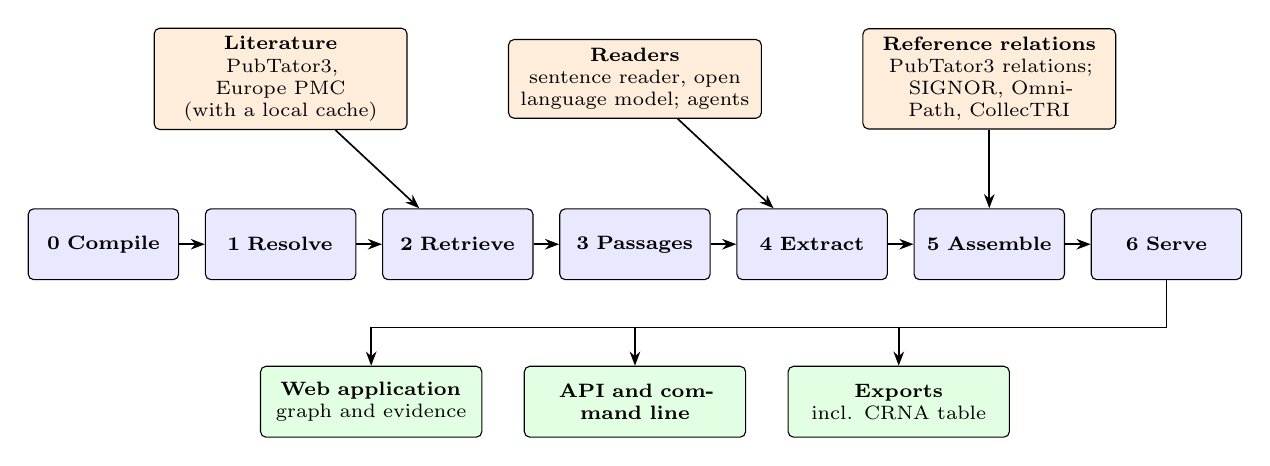
\begin{tikzpicture}[
    font=\scriptsize,
    box/.style={draw, rounded corners=2pt, align=center, inner sep=3pt},
    stage/.style={box, fill=blue!9, text width=1.7cm, minimum height=0.9cm},
    side/.style={box, fill=orange!14, text width=3.0cm, minimum height=1.0cm},
    sink/.style={box, fill=green!11, text width=2.6cm, minimum height=0.9cm},
    arr/.style={-{Stealth[length=1.8mm]}, semithick}]
  \foreach \col/\nm/\ttl in {0/compile/0 Compile, 1/resolve/1 Resolve, 2/retrieve/2 Retrieve,
                             3/passages/3 Passages, 4/extract/4 Extract, 5/assemble/5 Assemble,
                             6/serve/6 Serve}
    \node[stage] (\nm) at (\col*2.25, 0) {\textbf{\ttl}};
  \foreach \src/\dst in {compile/resolve, resolve/retrieve, retrieve/passages, passages/extract,
                         extract/assemble, assemble/serve}
    \draw[arr] (\src) -- (\dst);
  \node[side] (lit) at (2.25, 2.1) {\textbf{Literature}\\PubTator3, Europe PMC\\(with a local cache)};
  \node[side] (llm) at (6.75, 2.1) {\textbf{Readers}\\sentence reader, open\\language model; agents};
  \node[side] (db)  at (11.25, 2.1) {\textbf{Reference relations}\\PubTator3 relations;\\SIGNOR, OmniPath, CollecTRI};
  \draw[arr] (lit) -- (retrieve);
  \draw[arr] (llm) -- (extract);
  \draw[arr] (db) -- (assemble);
  \node[sink] (web) at (3.4, -2.0) {\textbf{Web application}\\graph and evidence};
  \node[sink] (api) at (6.75, -2.0) {\textbf{API and command line}};
  \node[sink] (exp) at (10.1, -2.0) {\textbf{Exports}\\incl. CRNA table};
  \draw[arr] (serve.south) -- ++(0,-0.6) -| (web.north);
  \draw[arr] (serve.south) -- ++(0,-0.6) -| (api.north);
  \draw[arr] (serve.south) -- ++(0,-0.6) -| (exp.north);
\end{tikzpicture}
\caption{The \gen{} pipeline and the components it draws on.}
\label{fig:arch}
\end{figure}

\begin{itemize}
  \item \textbf{0 Compile} reads any of the three input forms into one query specification.
    A question in plain language can be turned into a query by a language model and confirmed by
    the user.
  \item \textbf{1 Resolve} replaces gene aliases by official HGNC symbols~\cite{hgnc}.
  \item \textbf{2 Retrieve} finds papers through PubTator3~\cite{pubtator3} and Europe
    PMC~\cite{europepmc}, and keeps them in a local cache. For a gene list it takes the papers of
    each pair of query genes from PubTator3's file of text-mined relations (pair retrieval).
    Optionally, it reads the PMC full texts of papers PubTator3 holds only as abstracts.
  \item \textbf{3 Passages} selects the sentences that name two entities of the question.
  \item \textbf{4 Extract} turns sentences into claims: source, target, relation (activates,
    represses, regulates, binds), evidence type and cell line. A claim is accepted only if the
    sentences it cites exist, come from one passage and name both entities. There are two
    strategies. \code{fast}, the default for gene lists, reads every sentence with a
    BiomedBERT~\cite{biomedbert} classifier fine-tuned on RegulaTome~\cite{regulatome} (three
    copies trained with different random seeds, whose readings are averaged); a local
    open-weight language model decides the pairs the classifier is unsure of and gives a sign to
    links found without one. In wide mode a document reader trained on BioRED~\cite{biored} also
    proposes pairs from the whole abstract. \code{deep}, the default for topic queries, is a set of
    LangGraph~\cite{langgraph} researcher agents with a critic.
  \item \textbf{5 Assemble} merges claims into one network per cell line and marks conflicting
    signs. For \code{fast}, each signed edge is compared with the relations PubTator3's own model
    read for that pair across PubMed and gets a tier (Table~\ref{tab:tierdefs}). Each edge also
    says whether its sentences speak of the target's amount or its activity.
  \item \textbf{6 Serve} offers a web API with background jobs, a web application with 2D and 3D
    graphs and the evidence of every edge, a command line, and exports.
\end{itemize}

\begin{table}[htbp]
\centering
\small
\begin{tabularx}{\textwidth}{@{}lL@{}}
\toprule
\textbf{Tier} & \textbf{When an edge gets it}\\
\midrule
confirmed & \gen{}'s sign is the one PubTator3's relations for the pair clearly favour\\
probable & \gen{}'s sign, read in two or more papers, where PubTator3's relations favour no sign;
  or a sign taken from PubTator3's relations for a link \gen{} found unsigned\\
one-paper & as probable, but all its sentences come from one paper\\
reverse-only & a sign taken from PubTator3's relations for the pair the other way round\\
context-dependent & PubTator3's relations report both signs without a clear lean, or \gen{}'s own
  sentences state both\\
disputed & PubTator3's relations clearly favour the other sign; the edge keeps its direction, and
  its sign as a note\\
unsigned & a direction or a binding with no stated sign\\
\bottomrule
\end{tabularx}
\caption{The tiers of the \code{fast} strategy's edges. ``Clearly favour'': at least two relations
for one sign and twice as many as for the other. A sign taken from PubTator3's relations for an
unsigned link needs at least five. Apart from disputed edges, a tier flags a sign without
changing it.}
\label{tab:tierdefs}
\end{table}

All model calls go through one client for OpenAI-compatible servers, so the model
server (vLLM~\cite{vllm}, Ollama~\cite{ollama} or a hosted service for development) is a
setting. An evaluation harness compares components against baselines and decides which one is
used. CRNA stays a separate tool that exchanges only files with \gen{}: it is
written in R, a run takes minutes, and part of its source carries a research-only licence.

\textbf{Preparation and answering.} Fetching papers and reading them with a language model takes
minutes per cell line on the hardware we have. Our design therefore reads the papers of a topic
ahead of time and stores the checked claims, so that a later query on that topic only assembles
stored results. The six example topics are prepared first. A topic that has not been prepared is
answered more slowly, with the result marked as incomplete until its papers have been read.

\begin{table}[htbp]
\centering
\small
\begin{tabular}{@{}ll@{}}
\toprule
\textbf{Layer} & \textbf{Technology}\\
\midrule
Web application & React, TypeScript, Vite; Cytoscape.js (2D graph), three.js (3D graph)\\
API and jobs & Python, FastAPI, Pydantic; Celery workers with Redis\\
Storage & PostgreSQL with SQLAlchemy and Alembic; a local file cache for papers\\
Readers & LangGraph agents; open-weight models served by vLLM or Ollama; PyTorch\\
Deployment and quality & Docker Compose; pytest, ruff, mypy, ESLint; GitHub Actions\\
\bottomrule
\end{tabular}
\caption{Technology of each layer.}
\label{tab:tech}
\end{table}

\needspace{5\baselineskip}
\subsection{Constraints}

\needspace{5\baselineskip}
\subsubsection{Implementation Constraints}
\begin{itemize}
  \item Five students, two semesters, fixed course deadlines.
  \item PubTator3 is used at about three requests a second, the limit NCBI sets without a
    key~\cite{ncbikey}. A topic that has not been fetched before therefore needs tens of seconds
    of retrieval.
  \item The team has no dedicated GPU. Development uses laptops and free cloud GPUs (Kaggle, two
    T4 cards, about 30 hours a week) and one laptop GPU with 8\,GB of memory, which limits the
    size of the language model. On that GPU the sentence reader (1.4\,GB) and a
    4-billion-parameter language model (4.1\,GB) run together.
  \item No human-labelled data exists for our task, and the team has no labeller. Labels from
    curated databases are noisy. We therefore measure on corpora that others labelled by hand
    (RegulaTome~\cite{regulatome}, BioRED~\cite{biored}) and against experimental data, rather
    than labelling ourselves.
  \item Gene-list queries take 50 to 150 genes; input files are limited to 1\,MB on the
    command line and to 256\,KiB through the web API.
\end{itemize}

\needspace{5\baselineskip}
\subsubsection{Economic Constraints}
The project has no budget, and every resource it depends on is free: the GitHub free plan, free
cloud GPUs, public literature services, open-source software, and data that is free for research (some of it for academic use only,
Table~\ref{tab:sources}). Running
models locally avoids recurring per-query costs. A deployment needs one machine with Docker.

\needspace{5\baselineskip}
\subsubsection{Ethical Constraints}
\begin{itemize}
  \item A network is a set of hypotheses from the literature, not medical advice.
  \item No accuracy is claimed that has not been measured; comparisons with databases are
    reported as agreement.
  \item Several data sources (SIGNOR, OmniPath and the resources it integrates) carry their own
    licences, some for academic use only. \gen{} is used for academic research and credits its
    sources. Part of CRNA's source allows research use only, which is one reason CRNA stays
    outside the product.
  \item No personal or patient data is processed. With local models, queries are not sent to a
    model provider.
\end{itemize}

\begin{table}[htbp]
\centering
\small
\begin{tabularx}{\textwidth}{@{}lLL@{}}
\toprule
\textbf{Source} & \textbf{What \gen{} uses it for} & \textbf{Terms}\\
\midrule
PubTator3 (NCBI) & papers and entity annotations & public service; use paced to its limit\\
Europe PMC & abstracts for gene-list queries & public service; full text only when open
  access\\
HGNC & official gene symbols & CC0\\
TRRUST, SIGNOR, OmniPath, CollecTRI & comparison and training labels & per resource; some for
  academic use only\\
CRNA & downstream analysis, kept outside the product & GPL-3; part of its source for research
  use only\\
\bottomrule
\end{tabularx}
\caption{Data sources and their terms.}
\label{tab:sources}
\end{table}

\needspace{5\baselineskip}
\subsubsection{Other Constraints}
\begin{itemize}
  \item \textbf{Environmental:} papers and model answers are cached, so repeated topics cost
    little computation; small models are preferred over large ones.
  \item \textbf{Social:} users are biologists, not programmers, so the interface accepts plain
    questions and shows evidence instead of bare scores. The literature over-represents
    well-studied genes, and networks inherit this bias.
  \item \textbf{Political:} the literature services are operated by NCBI and EMBL-EBI; the local
    cache reduces the dependence on them.
  \item \textbf{Health and safety:} research use only; no patient data.
  \item \textbf{Manufacturability:} the stack starts with one command and uses pinned
    dependencies.
  \item \textbf{Sustainability:} automated tests, continuous integration and decision records keep
    the code maintainable; results record the model and data versions that produced them.
\end{itemize}

\needspace{5\baselineskip}
\subsection{Professional and Ethical Issues}

We follow the ACM Code of Ethics and Professional Conduct~\cite{acmcode}. The points below are the
ones that our project makes concrete.
\begin{itemize}
  \item \textbf{Honesty} (ACM 1.3). We report results with their baselines and their limits, and
    we report failures as well as successes. A number that compares our system only with a
    database is called agreement, not accuracy. The rule that decides each experiment is
    written down and committed before it runs, and the held-out queries are scored once per
    change, so that our results are not tuned to the data they are measured on.
  \item \textbf{Avoiding harm} (ACM 1.2). A wrong but convincing network could mislead a study.
    Every edge therefore shows the sentences it came from, edges with conflicting evidence are
    marked, and the interface states that the networks are for research only.
  \item \textbf{Credit and licences} (ACM 1.5). The system rests on the work of others:
    PubTator3, Europe PMC, HGNC, the curated databases, open-weight models and CRNA. We cite them
    and respect their terms of use.
  \item \textbf{Privacy and security} (ACM 1.6, 2.9). No personal data is processed. Secrets are
    kept out of the repository, only the component that calls the models receives the model
    settings, and inputs are checked and limited in size.
  \item \textbf{Competence} (ACM 2.6). We are computer engineers, not biologists. The system
    therefore makes no biological judgement of its own: it shows the evidence, and the researcher
    decides.
  \item \textbf{Teamwork.} The work is divided into five workstreams with named owners. Changes are
    reviewed through pull requests, the project board records who did what, and each member keeps
    a logbook.
\end{itemize}

\subsection{Standards}

\begin{table}[htbp]
\centering
\small
\renewcommand{\arraystretch}{1.1}
\begin{tabular}{@{}lll@{}}
\toprule
\textbf{Area} & \textbf{Standard} & \textbf{Where it is used}\\
\midrule
Modelling & UML 2.5.1~\cite{uml} & diagrams of the later reports\\
Requirements & ISO/IEC/IEEE 29148~\cite{iso29148} & numbered ``shall'' requirements\\
Web API & OpenAPI 3.1~\cite{openapi}, JSON Schema & API description, data contracts\\
Tables and graphs & CSV (RFC 4180), GraphML, CX & input files, exports\\
Gene names & HGNC symbols~\cite{hgnc} & names of gene nodes\\
Literature & PubMed identifiers, BioC & evidence links, annotated papers\\
Code & PEP 8, type checking & checked on every change\\
Version control & Git, reviewed pull requests & all code and documents\\
\bottomrule
\end{tabular}
\caption{Standards used in the project.}
\end{table}

The data formats that \gen{} reads and writes are all open and widely used. Gene-list queries
and the CRNA knowledge base (\code{source\_name}, \code{target\_name}, \code{sign},
\code{weight}) are CSV tables (RFC 4180~\cite{rfc4180}). The query specification and every result
of the API are JSON, with a schema generated from the code. Candidate graphs can be read as
GraphML~\cite{graphml}, an XML format for graphs, which is also planned as an export together with
CX~\cite{ndex}, the format of the NDEx repository, so that networks can be shared there.
PubTator3 returns papers in BioC~\cite{bioc}, a format for annotated biomedical text in which every
gene, chemical and cell line mention is marked. Genes are named by their official HGNC symbol, and
every piece of evidence points to its paper by its PubMed identifier (PMID).

\needspace{8\baselineskip}

% =====================================================================
\section{Design Requirements}
% =====================================================================

\needspace{5\baselineskip}
\subsection{Functional Requirements}\label{sec:fr}

Requirements are numbered and grouped by area; FR-32 to FR-36 were added on 20 November. The
last column gives the state on 20 November 2026: \textbf{B} built, \textbf{P} partly built,
\textbf{N} planned.

{\small
\begin{longtable}{@{}p{1.2cm}p{12.6cm}c@{}}
\toprule
\textbf{ID} & \textbf{The system shall \dots} & \textbf{State}\\
\midrule
\endfirsthead
\toprule
\textbf{ID} & \textbf{The system shall \dots} & \textbf{State}\\
\midrule
\endhead
\bottomrule
\caption{Functional requirements.}\label{tab:fr}
\endlastfoot
\addlinespace
\multicolumn{3}{@{}l}{\textbf{Query input}}\\
FR-1 & accept a topic query: a stimulus, one or more cell lines and the pathways of interest. & B\\
FR-2 & accept a disease with 50 to 150 genes as a CSV or JSON file. & B\\
FR-3 & accept a candidate graph as a CSV, JSON or GraphML file. & B\\
FR-4 & turn a question in plain language into a query that the user confirms before it runs. & B\\
FR-5 & reject malformed or oversized input with a message that names the cause. & B\\
FR-6 & replace gene aliases by official HGNC symbols, and report unknown and ambiguous names. & B\\
\addlinespace
\multicolumn{3}{@{}l}{\textbf{Retrieval and reading}}\\
FR-7 & retrieve papers from PubTator3 and Europe PMC, by search and for each gene pair of the
  query, and keep them in a local cache. & B\\
FR-8 & keep its requests to the literature services within their rate limits. & B\\
FR-9 & select the sentences that name two entities of the question. & B\\
FR-10 & extract signed, directed claims with their evidence type and cell line. & B\\
FR-11 & accept a claim only if its cited sentences exist, come from one passage and name both entities. & B\\
FR-12 & read every sentence with a fine-tuned sentence classifier, the main reader of the
  \code{fast} strategy. & B\\
FR-13 & read the papers of a listed topic ahead of time and store the checked claims. & P\\
FR-32 & read, on request, the PMC full texts of papers that PubTator3 holds only as abstracts. & B\\
FR-33 & offer a document reader that proposes pairs from a whole abstract, for the language model
  to decide (wide mode). & B\\
\addlinespace
\multicolumn{3}{@{}l}{\textbf{Networks}}\\
FR-14 & build one network per cell line. & B\\
FR-15 & mark an edge as a conflict when its papers disagree about the sign. & B\\
FR-16 & list the links whose sign differs between cell lines. & B\\
FR-17 & keep both directions of a feedback loop as separate edges. & B\\
FR-18 & list statements that a relation has no effect as counter-evidence. & B\\
FR-34 & give every edge a tier that says how far its sign is backed: by PubTator3's relations, by
  more than one paper, or disputed (Table~\ref{tab:tierdefs}). & B\\
FR-35 & say for every edge whether its sentences speak of the target's amount or its activity. & B\\
FR-36 & load SIGNOR, OmniPath, CollecTRI and STRING as prior relations with HGNC names, and answer
  pairs without papers from them. & P\\
\addlinespace
\multicolumn{3}{@{}l}{\textbf{User interface and API}}\\
FR-19 & show the network as a 3D graph, a 2D graph and a table, with filters. & B\\
FR-20 & show, for any edge, its sentences and the PubMed links of its papers. & B\\
FR-21 & show the current pipeline stage while a query runs. & B\\
FR-22 & let the user accept or reject an edge after reading its evidence. & N\\
FR-23 & offer a web API to submit a query, follow its progress and fetch the result. & P\\
FR-24 & offer a command line that runs any query through the pipeline. & B\\
FR-25 & let the user delete a submitted job and its result. & N\\
\addlinespace
\multicolumn{3}{@{}l}{\textbf{Export}}\\
FR-26 & export a network as a CRNA knowledge base with a manifest. & B\\
FR-27 & export a network as GraphML and CX. & N\\
\addlinespace
\multicolumn{3}{@{}l}{\textbf{Evaluation and records}}\\
FR-28 & compare a network with SIGNOR, OmniPath and CollecTRI. & B\\
FR-29 & score a result against gold relations, with coverage and precision together and next to a baseline. & B\\
FR-30 & record the stage times, model calls and model versions of every run. & B\\
FR-31 & measure how much two runs of the same query differ. & B\\
\end{longtable}}

Figure~\ref{fig:status} sums up the state of the 36 requirements. FR-36 is partly built: the
four sources load, with gene names mapped to HGNC symbols; answering from them is planned.

\begin{figure}[htbp]
\centering
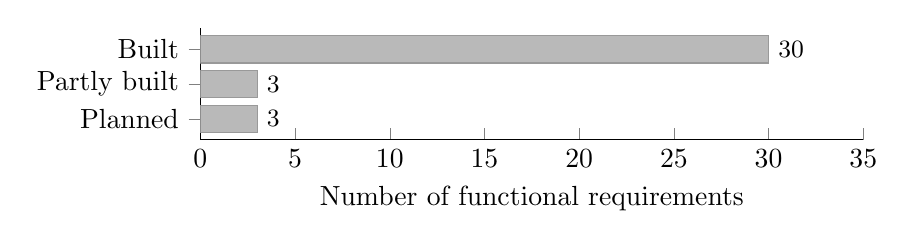
\begin{tikzpicture}
\begin{axis}[
  xbar, width=10cm, height=3.0cm, bar width=10pt, xmin=0, xmax=35,
  symbolic y coords={Planned, Partly built, Built}, ytick=data,
  xlabel={Number of functional requirements}, nodes near coords,
  enlarge y limits=0.3, axis x line*=bottom, axis y line*=left,
  every node near coord/.append style={font=\small}]
\addplot[fill=gray!55, draw=gray!80] coordinates {(30,Built) (3,Partly built) (3,Planned)};
\end{axis}
\end{tikzpicture}
\caption{State of the functional requirements on 20 November 2026.}
\label{fig:status}
\end{figure}

The minimum deliverable of the project is one complete path for estradiol in MCF-7 cells: a
network with visible evidence, its CRNA export, and its comparison with the curated databases.
Table~\ref{tab:deliverable} lists its parts.

\begin{table}[htbp]
\centering
\small
\begin{tabularx}{\textwidth}{@{}lLc@{}}
\toprule
\textbf{Part} & \textbf{What it needs} & \textbf{State}\\
\midrule
Network with evidence & the estradiol topic read, and every edge shown with its sentences
  (FR-9 to FR-11, FR-20) & B\\
User judgement & accepting or rejecting each edge in the web application (FR-22) & N\\
CRNA export & the network written as a CRNA knowledge base (FR-26) & B\\
Database comparison & the network compared with SIGNOR, OmniPath and CollecTRI (FR-28) & B\\
\bottomrule
\end{tabularx}
\caption{Parts of the minimum deliverable and their state.}
\label{tab:deliverable}
\end{table}

\needspace{6\baselineskip}
\subsection{Non-Functional Requirements}

\needspace{5\baselineskip}
\subsubsection{Usability}
\begin{itemize}
  \item A researcher shall be able to ask a question and see a network without programming.
  \item The evidence of any edge shall be reachable from the graph in at most two actions.
  \item Error messages shall name their cause, for example ``got 12 unique genes, expected
    50--150''.
  \item A question may be typed in plain language; it is shown back as a structured query to
    confirm before anything runs, with example questions to start from.
  \item While a query runs, the interface shall show its current stage.
  \item The sign of an edge shall not be shown by colour alone: activation is drawn with an
    arrowhead and repression with a bar.
\end{itemize}

\needspace{5\baselineskip}
\subsubsection{Reliability}
\begin{itemize}
  \item A failed call to a literature service or a model shall not fail the whole query; the
    result shall report what failed.
  \item A query that reaches its time limit shall return what it found, marked as incomplete.
  \item Every literature edge shall cite at least one sentence that names both of its entities.
  \item Every signed edge shall carry its tier, so that a user can keep only the most trusted
    signs: confirmed and probable edges agreed with the curated databases 94.1\% of the time on the nine
    held-out queries, one-paper edges 78.9\%.
  \item A doubtful sign shall be flagged by its tier, not deleted, so that no right sign is lost;
    a disputed edge keeps its sign as a note.
  \item A model call that is slow or fails shall be retried, or sent to a second model; a paper
    that a literature service refuses shall be skipped, not end the run.
  \item Cached files shall be written whole or not at all, so that a damaged file is never read.
\end{itemize}

\needspace{5\baselineskip}
\subsubsection{Performance}

\begin{figure}[htbp]
\centering
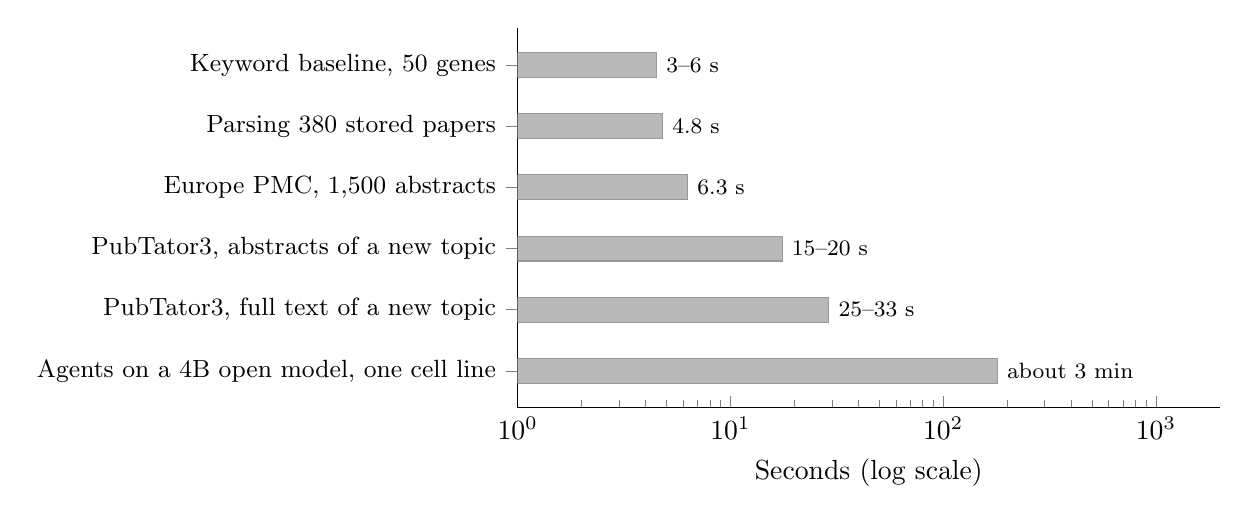
\begin{tikzpicture}
\begin{axis}[
  xbar, xmode=log, log basis x=10, width=10.5cm, height=6.4cm, bar width=9pt,
  xmin=1, xmax=2000, xlabel={Seconds (log scale)},
  symbolic y coords={Agents on a 4B open model{,} one cell line,
    PubTator3{,} full text of a new topic, PubTator3{,} abstracts of a new topic,
    Europe PMC{,} 1{,}500 abstracts, Parsing 380 stored papers, Keyword baseline{,} 50 genes},
  ytick=data, yticklabel style={font=\small, align=right}, nodes near coords,
  nodes near coords style={font=\footnotesize, anchor=west}, point meta=explicit symbolic,
  enlarge y limits=0.12, axis x line*=bottom, axis y line*=left]
\addplot[fill=gray!55, draw=gray!80] coordinates {
  (180,{Agents on a 4B open model{,} one cell line}) [about 3 min]
  (29,{PubTator3{,} full text of a new topic}) [25--33 s]
  (17.5,{PubTator3{,} abstracts of a new topic}) [15--20 s]
  (6.3,{Europe PMC{,} 1{,}500 abstracts}) [6.3 s]
  (4.8,{Parsing 380 stored papers}) [4.8 s]
  (4.5,{Keyword baseline{,} 50 genes}) [3--6 s]};
\end{axis}
\end{tikzpicture}
\caption{Measured times, from single runs on one machine: indications, not benchmarks. Ranges are
drawn at their midpoint, on a log scale. Reading with a language model dominates.}
\label{fig:times}
\end{figure}

Retrieval is limited by the request rate of the literature services, and reading by the speed of
the models on the hardware we have. Two measures cut the reader's time by more than two thirds
without losing signs
(Table~\ref{tab:speed}): the second and third copies of the reader only re-read the sentences the first
is unsure about, which are about 30\% of them, and every sentence's reading is stored and reused
by later queries. With both, reading the six example queries took 359 seconds instead of 1,283,
and repeating a query reads nothing again. The language model is now the slowest step. A whole
\code{fast} query of 63 to 130 genes takes about 4 minutes with its papers cached, and 10.8
minutes with nothing cached (15.8 in wide mode). Our goal
remains to answer a prepared query in about 30 seconds by reading its papers ahead of time.

\begin{table}[htbp]
\centering
\small
\begin{tabularx}{\textwidth}{@{}Lccc@{}}
\toprule
\textbf{Reader setting, six example queries} & \textbf{Reading time} & \textbf{Right / wrong sign} & \textbf{Sign agreement}\\
\midrule
Three reader copies read every sentence (before) & 1,283 s & 1,716 / 305 & 84.9\%\\
Copies two and three re-read only unsure sentences & 651 s & 1,720 / 292 & 85.5\%\\
The same, readings stored and shared across queries & 359 s & 1,719 / 292 & 85.5\%\\
The same, every sentence already stored & 4 s & 1,719 / 292 & 85.5\%\\
\bottomrule
\end{tabularx}
\caption{Reader speed on the 8\,GB laptop GPU, with the papers and language-model answers held
fixed. On the nine held-out queries the faster setting gave 2,132 right and 373 wrong signs, against
2,130 and 387 before.}
\label{tab:speed}
\end{table}

\needspace{5\baselineskip}
\subsubsection{Supportability}
\begin{itemize}
  \item Each pipeline stage is an interface with replaceable implementations.
  \item Every change passes continuous integration (style, types, 410 automated tests, build,
    dependency audit); the reading strategy has 65 tests of its own.
  \item Every new option of the reading strategy is off by default until it has been measured;
    options that did not help stay in the code, switched off, so that their results can be
    reproduced.
  \item All settings are environment variables; changing the model server needs no code change,
    and a check command reports what a model server cannot do.
  \item The architecture, the operations and the design decisions are documented in the
    repository, next to the code.
  \item Each folder of the code has a named owner who reviews changes to it.
\end{itemize}

\needspace{5\baselineskip}
\subsubsection{Scalability}
\begin{itemize}
  \item Queries run as background jobs, so several users can submit at the same time.
  \item Fetched papers and model answers are cached and reused between queries.
  \item Larger gene lists are a goal; the present limit is 150 genes. In tests outside that
    limit, gene lists of 250, 500 and 1,000 genes took 11, 34 and about 40 minutes, the last with
    the papers of the smaller runs already stored. Sentences grow faster than genes (90,000,
    820,000 and 2.3 million), and at 1,000 genes only 400 of 21,229 uncertain pairs fit within the
    language model's question limit, so large lists will need a job scheduler and a faster model.
\end{itemize}

\begin{table}[htbp]
\centering
\small
\begin{tabular}{@{}lll@{}}
\toprule
\textbf{Limit} & \textbf{Value today} & \textbf{Set by}\\
\midrule
Genes in a gene-list query & 50 to 150 & our input rules\\
Input file, command line & 1\,MB & our input rules\\
Web API request, uploads included & 256\,KiB & our input rules\\
Requests to PubTator3 & about 3 a second & NCBI's limit without a key\\
Free GPU time & about 30 hours a week & Kaggle\\
How long a result is kept & 7 days & our settings\\
\bottomrule
\end{tabular}
\caption{Current limits of the system.}
\label{tab:limits}
\end{table}

\needspace{5\baselineskip}
\subsubsection{Portability}
\begin{itemize}
  \item The whole system starts with one command (\code{docker compose up}) on one machine, as five
    services: the database (PostgreSQL), the job queue and result store (Redis), the API, a worker
    that runs the pipeline, and the web interface.
  \item The official gene-name table is built into the image, so name resolution needs no network
    call.
  \item The language model is reached through an OpenAI-compatible interface, so the same code runs
    against a local model server such as Ollama~\cite{ollama} or vLLM~\cite{vllm} on a laptop, a lab
    server or a free GPU.
  \item Data and results are kept in named volumes and survive a restart of the services.
\end{itemize}
\needspace{8\baselineskip}

% =====================================================================
\section{Feasibility Discussions}
% =====================================================================

\needspace{5\baselineskip}
\subsection{Market \& Competitive Analysis}

\needspace{5\baselineskip}
\subsubsection{Target Users}

\gen{} is meant for researchers who study how cells respond to a stimulus or how genes are
regulated in a disease, and who need a signed, directed network for their question:
\begin{itemize}
  \item \textbf{Experimental biologists} who want to know what the literature says about a
    stimulus in their cell line before they plan an experiment, without reading every paper by
    hand. They usually do not program.
  \item \textbf{Computational biologists} who run causal analysis methods, such as CRNA, on their
    own expression data and need a knowledge base that fits their cell line. Our first users are
    in this group: the group of our innovation expert, which develops CRNA.
  \item \textbf{Students and research groups without a commercial licence}, who cannot use
    commercial knowledge bases.
\end{itemize}
What these users lack today is a quick way from a question to a network whose every edge they can
check against its source.

\needspace{5\baselineskip}
\subsubsection{Market Research}

The amount of literature grows faster than anyone can read it. PubMed added about 1.57 million
citations in the 2023 fiscal year alone and held about 36.6 million in total~\cite{nlmstats}.
Answering a question about a few dozen genes therefore means searching a body of text that no
researcher can cover by hand.

The market for software that turns biological data into knowledge is large and growing. One
estimate puts the global bioinformatics market at about \$20.9 billion in 2024 and
\$43.5 billion by 2030, a growth of about 13\% a year~\cite{bccbioinfo}. Pathway analysis, the use
that \gen{}'s networks serve, is estimated at about \$5.2 billion in 2025 and growing by about
20\% a year~\cite{gvrpathway}. Such estimates differ between publishers, because they define the
market differently, so we read them as a sign of demand rather than as exact figures. The paid
products in this market, such as Ingenuity Pathway Analysis~\cite{ipa}, are licensed, which leaves
a gap for free tools that research groups can run themselves.

\needspace{5\baselineskip}
\subsubsection{Competitive Analysis}

\begin{table}[htbp]
\centering
\small
\begin{tabularx}{\textwidth}{@{}lLl@{}}
\toprule
\textbf{Tool} & \textbf{What it is} & \textbf{Access}\\
\midrule
SIGNOR 3.0~\cite{signor} & manually curated causal relations with sign and direction & free\\
OmniPath~\cite{omnipath} & integration of more than 100 resources into signed networks & free\\
STRING 12.5~\cite{string} & protein networks, with a regulatory network read from the
  literature by a fine-tuned model & free\\
PubTator3~\cite{pubtator3} & entity and relation annotations over PubMed & free\\
INDRA~\cite{indra} & assembles statements from text-mining readers and databases into causal
  models & free\\
Ingenuity Pathway Analysis~\cite{ipa} & commercial knowledge base with causal analysis &
  licensed\\
\bottomrule
\end{tabularx}
\caption{Related tools.}
\end{table}

Most capabilities of \gen{} exist individually in these tools. Curated databases are precise but
built once, for all contexts, and they cover only what their curators have read. Whole-proteome
resources such as STRING give the full network rather than the one for a chosen stimulus and cell
line. Commercial products are licensed and closed. INDRA is the closest in aim, but it is a
programming library for model builders. What \gen{} combines is a network built for one question
and separated by cell line, the evidence sentence on every edge, reading with local open models at
no licence cost, and an export for CRNA. Curated relations remain more reliable than
automatically read ones, so \gen{} does not replace the databases. Against the other readers,
however, we have measured a gain (Section~\ref{sec:prelim}): on the papers \gen{} read, INDRA's
readers found 1,092 of 3,843 curated links, and 30\% of their signed edges contradict the
databases; \gen{} found 2,698, and 12\% of its signed edges contradict them. On nine held-out queries, against all of INDRA's
literature, \gen{} gets as many signs right and has 115 to 210 fewer wrong (95\%); its
confirmed and probable signs agree with the databases 94.1\% of the time.
\gen{} is an academic research tool and has no commercial plan.

\needspace{5\baselineskip}
\subsection{Academic Analysis}

\needspace{5\baselineskip}
\subsubsection{Knowledge Bases for Causal Analysis}

Regulatory networks are built in two ways. Methods such as GENIE3~\cite{genie3} infer them from
expression data alone. Causal reasoning methods start from prior knowledge instead: they take a
signed, directed network and ask which regulators explain a measured expression change. Examples
are PARADIGM~\cite{paradigm}, the causal analysis of Ingenuity Pathway Analysis~\cite{ipa},
CausalR~\cite{causalr} and CRNA~\cite{crna}. The quality and the context of their knowledge base
bound what they can find. Today that knowledge base comes from curation, as in
SIGNOR~\cite{signor} and TRRUST~\cite{trrust}, or from integrating curated resources, as in
OmniPath~\cite{omnipath} and CollecTRI~\cite{collectri}. \gen{} adds a knowledge base read from the
literature for one question and one cell line.

\needspace{5\baselineskip}
\subsubsection{Reading Relations from Text}

Reading relations automatically from papers is feasible, and recent work shows both its reach and
its limits. PubTator3 marks entities and extracts typed relations over the whole of PubMed with
a transformer model, BioREx~\cite{pubtator3, biorex}. RegulaTome is a corpus of 16,961 typed,
directed and signed relations annotated by hand in 2,521 documents; a fine-tuned model reached an
F1 score of 66.6\% on it~\cite{regulatome}. STRING 12.5 fine-tuned a model on this corpus, reports
an F1 score of 73.5\%, and ran it over all PubMed abstracts and open-access full texts to build its
regulatory network~\cite{string}. Its reported precision is 75.2\%, so about a quarter of what
even such a model extracts is wrong, which is why \gen{} shows the evidence of every edge. INDRA collects statements
from several such readers and estimates how reliable each statement is; its authors found that
statements supported by many sentences can still be wrong, because readers make systematic
errors~\cite{indra, indra2023}.

\needspace{5\baselineskip}
\subsubsection{Labels and Model Training}

A model that reads sentences needs labelled sentences to learn from. Labels taken from a curated
database for every sentence of a cited paper, known as distant supervision~\cite{mintz}, are
plentiful but noisy, because a database cites a paper for a relation, not a sentence. A large model
can label data for a small one, known as distillation~\cite{hinton}, so that the expensive model
works only once and offline. Domain encoders pretrained on biomedical text, such as
BiomedBERT~\cite{biomedbert}, are a common starting point for the small model. \gen{} follows this
path in part: its sentence classifier is a fine-tuned BiomedBERT, but because database labels
proved too noisy, it is trained on the hand-annotated RegulaTome corpus instead, and measured on
RegulaTome's held-out test split.

\needspace{5\baselineskip}
\subsubsection{Preliminary Results}\label{sec:prelim}

\paragraph{The sentence reader.} The reader is BiomedBERT~\cite{biomedbert} fine-tuned on
RegulaTome~\cite{regulatome}, three copies trained with different random seeds and averaged, with a calibrated confidence for each edge.
Table~\ref{tab:prelim} gives its results on hand-annotated text and on our own papers.

\begin{table}[htbp]
\centering
\small
\begin{tabularx}{\textwidth}{@{}LccL@{}}
\toprule
\textbf{Method and data} & \textbf{Answered} & \textbf{Right} & \textbf{Limit}\\
\midrule
``Always activates'' on 115 known pairs among 50 breast-cancer genes & 100\% & 65.2\% & a
  baseline, no reading\\
Keyword rules on the same 115 pairs & 36.5\% & 33.3\% & do not beat the baseline\\
Reader on the RegulaTome test split, sentences read with confidence $\geq 0.95$ & 222 sentences &
  86.9\% (95\% CI 81.9--90.8\%) & hand labels, but the corpus the reader was trained on\\
Reader on 2,529 papers fetched by \gen{} runs, confident edges with a database sign & 1,370 edges
  & 93.7\% & database labels; agreement, not accuracy\\
\bottomrule
\end{tabularx}
\caption{Preliminary measurements. ``Right'' is the share of answers that match the label. The
rows use different data and cannot be compared with each other.}
\label{tab:prelim}
\end{table}

\paragraph{Whole networks against existing tools.} The \code{fast} strategy lets the reader decide
the pairs it reads with confidence $\geq 0.70$ and asks a local 4-billion-parameter model about the
uncertain ones. A further step asks the model for the sign of links found without one (``binds'' or
``regulates''), or to answer that the sentences state none. Two last steps compare each pair with
the relations PubTator3's own model read for it across all of PubMed. A link still without a sign
takes the sign those relations favour by a stricter rule than the one used for tiers: at least
five relations, and twice as many as for the other sign. A signed link whose sign they clearly
contradict, by the rule of Table~\ref{tab:tierdefs}, becomes disputed: it keeps its direction and
its sign only as a note, since such signs proved
right only about half the time; both rules were chosen on the six example queries. Its papers come
from pair retrieval: the three newest
papers of each pair of query genes in PubTator3's relation file~\cite{pubtator3}, and seven more for
each pair still without a confident signed reading. Table~\ref{tab:tools} compares the networks
for the six example queries with PubTator3, STRING~\cite{string} and INDRA~\cite{indra2023}. Every
tool is scored the same way, against the 3,843 links that SIGNOR, OmniPath and CollecTRI record
among the query genes. For INDRA we keep only evidence from its text-mining readers, since SIGNOR
is part of the reference. Here and below, a sign is called right when it matches the databases'
sign and wrong when they record the other one. The databases contain errors of their own (see the
audit below), so ``right'', ``wrong'' and ``sign agreement'' measure agreement, not accuracy.

\begin{table}[htbp]
\centering
\small
\begin{tabularx}{\textwidth}{@{}Lccc@{}}
\toprule
\textbf{Tool} & \textbf{Links found} & \textbf{Right / wrong sign} & \textbf{Contradicts databases}\\
\midrule
STRING text mining, score $\geq 0.4$ (no sign or direction) & 2,887 & -- & --\\
INDRA readers, all literature & 2,649 & 1,618 / 447 & 27\%\\
\textbf{\gen{} \code{fast}, pair retrieval} & \textbf{2,698} & \textbf{1,779 / 252} & \textbf{12\%}\\
\gen{} \code{fast}, wide mode & 2,741 & 1,797 / 256 & 12\%\\
\gen{} \code{fast} without the two PubTator3 steps & 2,697 & 1,720 / 292 & 15\%\\
\gen{} reader alone, pair retrieval & 2,300 & 1,081 / 145 & 12\%\\
STRING text mining, score $\geq 0.7$ (no sign or direction) & 1,371 & -- & --\\
INDRA readers, the same papers as \gen{} & 1,092 & 522 / 157 & 30\%\\
PubTator3 relations & 249 & -- & --\\
\bottomrule
\end{tabularx}
\caption{Six example queries, 3,843 curated links. ``Contradicts databases'' is the share of a
tool's signed edges whose sign a database records the other way. Where INDRA states both signs
for a link, the sign more of its papers state is kept; where they tie, both are kept as two edges,
one of which contradicts, so for INDRA this share is higher than wrong / (right + wrong). These
runs predate the fixes that followed the audit of wrong signs (below), after which \gen{}
\code{fast} gives 1,781 right and 248 wrong. The database labels are incomplete, so these figures
are agreement, not accuracy.}
\label{tab:tools}
\end{table}

Against INDRA's whole literature, \gen{} finds more links (2,698 against 2,649), more with the
right sign (1,779 against 1,618) and fewer with the wrong one (252 against 447), and it contradicts
the databases less than half as often. A bootstrap over the links puts the difference in right
signs between +95 and +228 and in wrong signs between $-239$ and $-151$ (95\%). On the same papers,
\gen{} finds 2.5 times INDRA's links. Pair retrieval accounts for most of the gain in links: the
agents' disease searches gave 967. With its papers cached, \code{fast} takes about four minutes per
query on the 8\,GB laptop GPU.

\paragraph{Held-out queries.} The thresholds and rules were chosen on these six queries, so they
flatter \gen{}. Nine more queries, built from other SIGNOR pathways and never used to choose
anything, give 4,587 curated links (Table~\ref{tab:heldout}). On them \gen{} gets as many signs
right as INDRA and far fewer wrong, and its sign agreement is higher with 95\% intervals that do
not overlap. Of the two PubTator3 steps, the first adds right signs and the second removes wrong
ones. With the first alone, \gen{} gets 69 to 214 more signs right than INDRA, and 93 more right but
102 more wrong than with both; we keep both, preferring fewer wrong signs.
In wide mode, a document reader that sees the whole abstract also proposes pairs the sentence
reader left unlinked, and the language model decides each (it added 73 to 210 links per held-out query).
\gen{} then gets more signs right than INDRA (2,245 against 2,162, $+12$ to $+155$) as well as
fewer wrong, with the same sign agreement as without wide mode, so it is ahead of INDRA on all
three measures. Measured with no
cached answers on the six example queries, wide mode takes 15.8 minutes per query against 10.8
(+46\%); all of the extra time is the document step.

\begin{table}[htbp]
\centering
\small
\begin{tabularx}{\textwidth}{@{}Lccc@{}}
\toprule
\textbf{System, nine held-out queries} & \textbf{Right / wrong sign} & \textbf{Sign agreement (95\%)} & \textbf{Right, \gen{} -- INDRA}\\
\midrule
\textbf{\gen{} \code{fast}} & \textbf{2,211 / 307} & \textbf{87.8\% (86.6--89.1)} & $-22$ to $+122$\\
\textbf{\gen{} \code{fast}, wide mode} & \textbf{2,245 / 318} & \textbf{87.6\% (86.4--88.9)} & $+12$ to $+155$\\
\gen{} \code{fast}, first PubTator3 step only & 2,304 / 409 & 84.9\% (83.6--86.3) & $+69$ to $+214$\\
\gen{} \code{fast} without the PubTator3 steps & 2,132 / 373 & 85.1\% (83.8--86.5) & $-107$ to $+42$\\
INDRA readers, all literature & 2,162 / 469 & 82.2\% (80.7--83.6) & \\
\bottomrule
\end{tabularx}
\caption{Nine held-out queries, 4,587 curated links; intervals from a bootstrap over the links.
Wrong signs, \gen{} minus INDRA: $-210$ to $-115$ for \code{fast}, $-201$ to $-103$ in wide
mode.}
\label{tab:heldout}
\end{table}

Agreement with PubTator3 also tells how far to trust a signed link. Where the sign \gen{} read and
the sign PubTator3's relations favour agree, it matched the databases 96.0\% of the time on the six
queries and 94.3\% on the held-out ones (1,374 links); where PubTator3 has no clear sign, 79\%.
These became the confirmed and probable tiers (Table~\ref{tab:tierdefs}); the later tiers, below,
split the less reliable links off the probable one. INDRA's corpus stops at an earlier
date, so we also restricted \gen{}'s papers and PubTator3's relations to the papers INDRA could
have read: on the six queries, 1,561 right and 253 wrong signs against INDRA's 1,618 and 447, a
tie in right signs ($-123$ to $+8$), 150 to 237 fewer wrong, and a sign agreement of 86.1\%
(84.4--87.6) against 78.4\% (76.5--80.2). A smaller language model, granite4.1 with 3 billion parameters, gave nearly the
same held-out result (2,215 right, 343 wrong) with the language-model steps about three times
faster.

\paragraph{Labels made by others.} No team member can label edges, so we use BioRED~\cite{biored},
600 abstracts in which NCBI curators labelled every relation between the genes they annotated
(Table~\ref{tab:biored}). Each system finds the genes with its own entity recognition. The INDRA
corpus we use covers only 64 of the abstracts and its web service was unavailable, so INDRA's
recall here is a lower bound.

\begin{table}[htbp]
\centering
\small
\begin{tabularx}{\textwidth}{@{}Lcccc@{}}
\toprule
\textbf{System} & \textbf{Abstracts} & \textbf{Precision} & \textbf{Recall} & \textbf{F1}\\
\midrule
\gen{} \code{fast} & 600 & 0.87 & 0.05 & 0.10\\
INDRA readers & 600 & 0.56 & 0.12 & 0.20\\
\midrule
\gen{} \code{fast} (test split) & 100 & \textbf{1.00} & 0.04 & 0.07\\
\textbf{\gen{} \code{fast}, wide mode (test split)} & 100 & \textbf{1.00} & 0.37 & \textbf{0.54}\\
\gen{} document reader alone (test split) & 100 & 0.64--0.81 & \textbf{0.49--0.52} & \textbf{0.56--0.62}\\
INDRA readers (test split) & 100 & 0.92 & 0.12 & 0.21\\
PubTator3 BioREx, trained with BioRED (test split) & 100 & 0.98 & 0.49 & 0.65\\
\bottomrule
\end{tabularx}
\caption{Gene--gene relations in BioRED. Precision: the share of a system's claims that the
curators labelled. Recall: the share of the labelled relations a system finds. The document reader
is shown as the range over three training seeds.}
\label{tab:biored}
\end{table}

The sentence reader of \code{fast} is precise, with nearly nine in ten of its claims labelled
relations, but it finds few. BioRED's relations are nearly always stated within one sentence (99\%
of related pairs, by BioRED's own gene labels), but PubTator3, whose gene marks the reader uses,
marks both genes of that sentence for only 224 of these 480 relations (47\%); gene recognition,
not the length of the evidence, limits the sentence reader. Reading only the closing summary sentences, where papers
often state their conclusion, found a third as many relations. BioRED also
labels correlations (``reduced MMP-9 after LDHA knockdown''), which the reader was trained not to
read as regulation. A document reader that reads the whole abstract, trained on BioRED's training
split only and scored once on its test split, reaches F1 0.56--0.62, three times INDRA's and close
to BioREx, PubTator3's model trained on BioRED. In \code{fast}'s wide mode, that reader proposes
pairs and the language model decides each, as in the product. On the test split this gives F1 0.54,
two and a half times INDRA's: all 38 of its claims are labelled relations, it finds 37\% of them,
and 24 of 30 signs are right. The test split has 103 relations, so these figures are uncertain
by several points.

We also compared signed edges with a genome-wide CRISPR screen in K562 cells~\cite{perturbseq}.
There, even the curated databases agree with the measured expression changes no more often than
``always activates'' does, so the screen cannot judge signs for any system, and we do not use it
to judge signs. We use it instead to test cell-line networks, below.

\paragraph{Knockdown experiments.} To test whether separating evidence by cell line helps, we
built regulons (each transcription factor's signed targets) for the cell line of each knockdown
experiment in KnockTF~\cite{knocktf}, pooling papers about the same line, the same disease, the
same organ and other lines with declining weights. A good regulon should rank the knocked-down
factor's activity among the most reduced, as estimated with decoupler~\cite{decoupler}. We split
KnockTF by study before tuning anything, fixed every setting on the development studies, and
committed a hash of the test set's experiment IDs. We then scored the test set (111 experiments,
88 studies, 80 cell lines) once. Separating by cell line and keeping signs both point the right way
($-0.028$ and $-0.014$ in rank percentile, lower is better), but neither is significant (95\%
intervals $-0.069$ to $+0.015$ and $-0.051$ to $+0.022$). Adding \gen{}'s edges to CollecTRI
changed nothing, and \gen{}'s regulons alone rank the factor worse than CollecTRI does (0.386
against 0.311). Most test lines have little literature of their own (a median of 49 papers that
name the line, against 137 on development), so the cell-line claim remains unproven. Testing it
again needs new experiments, because this test set is now used up.

\paragraph{A frozen test for cell-line networks.} CRISPRi screens that knock down the same genes
in K562, RPE1, HepG2 and Jurkat cells~\cite{perturbseq,nadig} measure what KnockTF could not: the
same knockdown in several cell lines. Before building any network for these lines, we split the
460 transcription factors that were knocked down effectively, with a measurable effect, into
development (30\%) and test (the other 70\%, by design: settings are tuned on development, and
the larger test is scored once), and committed a hash of the test set with the protocol. The
test has 305 knockdowns in K562's genome-wide screen and 55 factors usable in two or more lines.
It asks whether \gen{}'s network for a line changes where the measured response changes,
scored as F1 next to its chance level and next to a baseline that uses only which genes each
line expresses.

\paragraph{Hand-off to CRNA.} \gen{} now writes each network as a CRNA knowledge base with a
manifest (FR-26). For the estradiol network in MCF-7 cells, 1,689 signed links among genes
measured in the estradiol study GSE11352 go to CRNA. As an independent check, we compared those
links with that study. For links whose two genes both changed, the changes agreed with the link's
sign 53\% of the time (45--61\%), against 44\% for ``always activates'' and 48\% for random
signs. Moving together is thus too weak a test to confirm signs on one study, which is why
CRNA's result is reported as agreement, not as ground truth.

\paragraph{Auditing the wrong signs.} We read the 252 wrong signs on the six queries, and a
control of 100 right ones, with rules written down before any link was read. 80 are \gen{}'s own
errors: mostly a sign taken from the relation in the other direction, or ``knockdown of A lowered
B'' read as inhibition. 83 look like database errors (\gen{}'s sentences state its sign and none
states the databases'), and 87 are a sign that depends on the cell or condition, or a different
meaning of sign (activity against amount); 2 could not be decided. Only 2 of the 41 wrong signs among confirmed links are
\gen{}'s own errors. So, rather than drop doubtful signs, \gen{} now gives them tiers of their own:
\emph{reverse-only} (a PubTator3 sign on a pair already signed the other way round) and
\emph{context-dependent} (PubTator3's relations report both signs). No right sign is lost, and
confirmed and probable links together reach 91.9\% on the six queries and 90.0\% on the held-out
ones, from 87.6\% and 87.8\%. The context-dependent links are the least reliable on both sets
(61\% and 72\%). Each link also says whether its sentences speak of the target's amount or its
activity; where that matches SIGNOR's own label, 94\% of signs are right. One annotator who knew
which signs were wrong made these calls, so we checked them twice. In the full texts the databases
cite, a model found the databases' sign for 28 of 35 right pairs but for only 4 of 24 ``database
wrong'' pairs; 17 of those 24 stand. A model reading 50 audited links blind agreed with the audit
at Cohen's $\kappa = 0.50$. Counting the 83 database errors as right raises the share of right
signs among all signed links from 87.6\% to 91.7\%; discounting the verdicts the full texts overturned, it is
about 90.5\%. Knockdown experiments could not referee: on links
whose sign nobody disputes, they agree with it 64\% of the time against 60\% for ``always
activates''.

\paragraph{A validated model annotator.} No person can read the links blind, so we tested whether
open models can stand in, with a pass mark fixed beforehand: Cohen's $\kappa \geq 0.80$ against
RegulaTome's curators on 180 sentence sets, deciding at least 70\% of them. No single model passed
(the best, qwen3.5 with 35 billion parameters, reached 0.76). A jury of three local models
(qwen3.5:35b-a3b, gemma4:26b and gpt-oss:20b) that counts only unanimous readings reached 0.85
(0.76--0.91) and decided 81\% of the sets. This jury re-read the 352 audited links and 200 links
sampled from the held-out queries, which nobody had audited. It agrees with the audit: it reads
\gen{}'s sign for 71 of the 83 ``database wrong'' links and the databases' sign for none of them.

\paragraph{Papers per sign.} A sign stated in two or more papers is far more often right
(Table~\ref{tab:tiers}). Probable signs from a single paper agree with the databases 11 and 16
points less often than those from two or more, beyond the 5 points on both query sets that the rule written
beforehand asked for. They now form a tier of their own, \emph{one-paper}, which keeps the sign.
Confirmed and probable links then reach 95.6\% on the six queries and 94.1\% on the held-out ones;
the cost is that 23--30\% of their right signs move to the new tier. INDRA's signs gain from a
second paper too (from 69--72\% for signs from one paper to 81--86\% for two or more), so this is a property of signs read from the
literature, but \gen{} agrees more often at every cut. Counting a link as right where the jury
reads \gen{}'s sign in its sentences, confirmed and probable links on the held-out queries are
97.8\% right (96.8--98.8); counting as wrong also every right link whose sentences the jury finds
no sign in, 96.3\%.

\begin{table}[htbp]
\centering
\small
\begin{tabularx}{\textwidth}{@{}Lcc@{}}
\toprule
\textbf{Signed links} & \textbf{Six example queries} & \textbf{Nine held-out queries}\\
\midrule
\gen{}, all & 1,781 / 248 (87.8\%) & 2,211 / 307 (87.8\%)\\
\gen{}, confirmed + probable, before the one-paper tier & 1,546 / 136 (91.9\%) & 1,898 / 210 (90.0\%)\\
\textbf{\gen{}, confirmed + probable} & \textbf{1,082 / 50 (95.6\%)} & \textbf{1,454 / 91 (94.1\%)}\\
\gen{}, one-paper & 464 / 86 (84.4\%) & 444 / 119 (78.9\%)\\
\gen{}, any tier, two or more papers & 480 / 12 (97.6\%) & 648 / 17 (97.4\%)\\
INDRA readers, all & 1,618 / 447 (78.4\%) & 2,162 / 469 (82.2\%)\\
INDRA readers, two or more papers & 1,259 / 288 (81.4\%) & 1,675 / 277 (85.8\%)\\
\bottomrule
\end{tabularx}
\caption{Right / wrong signs against SIGNOR, OmniPath and CollecTRI as they are: agreement, not
accuracy. \gen{}'s figures
are the current default, after the audit's fixes; Table~\ref{tab:tools} gives the run before them
(1,779 / 252 on the six queries). No sign is deleted: a tier flags a sign, and a
disputed edge keeps its sign as a note.}
\label{tab:tiers}
\end{table}

\paragraph{What did not help.} Each of these was decided by a rule written before it ran, and
scored once on the held-out queries where the example queries allowed. Using the jury as a sign
check in the pipeline gained 1.0 point, but the links it rejects are still 68\% right: it reads
``no effect stated'' where the sign is right. Promoting context-dependent links the jury reads with
\gen{}'s sign gave links only 61\% and 74\% right, since their sentences do state the sign, for
other cells or conditions. Reading PMC full texts where PubTator3 holds only abstracts added
right signs but lowered held-out sign agreement by 0.3 points, whether the full-text sentences went to
every step or to the sentence reader only. Flagging hedged sentences (``may'', ``could''), giving
the language model one sentence per paper, and the reader's confidence within one-paper signs did
not separate right from wrong signs on both sets. Asking the language model each question three
times, with the sentences in different orders, did not help either. A second reading of the same sentences cannot
tell a context difference from a database error; an independent source, PubTator3's relations or
a second paper, can.

\paragraph{Next steps.}
\begin{itemize}
  \item \textbf{Ground truth.} A third of the signs counted wrong are database errors, and a
    further third differ by context or by what the sign means. Score every run against a
    corrected answer key, with the sentences behind each correction, and report it three ways:
    as the databases are, corrected and strict. Flag likely context and sign-meaning cases by
    code before anyone reads them.
  \item \textbf{Why the models decide as they do.} Record the cue behind each language-model
    decision and measure which cues (loss-of-function wording, negation, reverse direction)
    predict a wrong sign, for the sentence reader, the language-model steps and the jury.
  \item \textbf{Cell lines in the main network.} Choose the cell-line weighting on the
    Perturb-seq development factors only, and build one network per requested cell line in the
    main pipeline, not only in the benchmarks. Then run the frozen Perturb-seq test once.
  \item \textbf{Wide mode.} By a rule committed before it ran, wide mode stays an option, not the
    default (22 November): of the links it adds to the estradiol network, only 11 could be checked
    against the expression study, fewer than the 30 the rule required. Next, let it read results
    sections and supplementary tables, not only abstracts, which should add enough links to ask
    the question again under a new rule.
  \item \textbf{More evidence per sign.} Find second papers for one-paper signs; recognise the
    genes PubTator3 leaves unmarked, the limit found on BioRED; rank full-text sentences by
    section before they reach the language model.
  \item \textbf{Oncogenic signalling pathways.} Build \gen{} networks for the ten oncogenic
    signalling pathways curated by The Cancer Genome Atlas~\cite{tcgapathways}, score them against
    the pathways' signed templates, and export them for cancer genome analysis.
  \item \textbf{The application.} Run the \code{fast} strategy from the web application and show
    each edge's tier, cited sentences and cell-line differences; export GraphML, Cytoscape CX and
    JSON beside CRNA's knowledge base; run CRNA on the estradiol and EGF studies. Make queries
    faster, toward about 30 seconds, by reading the papers of every gene pair ahead of time.
\end{itemize}
\clearpage

% =====================================================================
\section{Glossary}
% =====================================================================

\begin{description}[leftmargin=0.6cm, itemsep=0.2em]
  \item[Activation, repression] The two signs of a relation: the source raises, or lowers, the activity, expression or level of the target.
  \item[Agent] A program in which a language model chooses its next step, such as which passages to read, whether to search again and when to stop.
  \item[BiomedBERT] A language-understanding model of about 110 million parameters, pretrained on biomedical text, which we fine-tune as a sentence classifier.
  \item[BioRED] A corpus of 600 PubMed abstracts in which NCBI curators labelled every relation between the entities they annotated; we use it to measure how many relations a reader finds.
  \item[Cell line] A population of cells grown in the laboratory, such as MCF-7 (breast cancer). The same stimulus can act differently in two cell lines.
  \item[Claim] One statement read from one passage: source, target, relation, evidence type and cell line.
  \item[Cohen's kappa ($\kappa$)] Agreement between two annotators beyond what chance would give: 1 is full agreement, 0 chance.
  \item[Conflict] An edge for which some papers report activation and others repression.
  \item[CRNA] Causal Regulatory Network Analysis, the R package of our innovation expert's group. It combines a signed knowledge base with expression data to infer active regulators.
  \item[Curated database] A collection of relations entered by people who read the papers, such as SIGNOR, OmniPath and CollecTRI.
  \item[Edge] A relation between two nodes of a network, with its direction, sign and evidence.
  \item[Evidence] The sentences, with their PubMed identifiers, from which an edge was read.
  \item[F1 score] The harmonic mean of precision (the share of a system's claims that are right) and recall (the share of the true relations it finds).
  \item[Gene regulatory network] A signed, directed graph of regulatory relations between genes and gene products.
  \item[Held-out queries] Nine queries never used to choose any setting, so that results on them are not tuned to them.
  \item[HGNC] The HUGO Gene Nomenclature Committee, which assigns official human gene symbols.
  \item[INDRA] An open system that assembles statements from several text-mining readers and databases into causal models; the closest existing tool, which we compare against.
  \item[Jury] Three open language models that read the same sentences; a reading counts only when all three agree.
  \item[KnockTF] A database of gene expression measured after a transcription factor is knocked down or knocked out, in many cell lines.
  \item[Knowledge base] The set of known signed, directed relations that a causal analysis method such as CRNA starts from.
  \item[Open-weight model] A language model whose weights can be downloaded and run on one's own hardware.
  \item[Pair retrieval] Taking the papers of each pair of query genes from PubTator3's file of text-mined relations.
  \item[Pathway] A named group of genes that act together, such as PI3K/AKT or MAPK/ERK.
  \item[Perturb-seq, CRISPRi] Experiments that switch off one gene per cell (CRISPR interference) and measure the expression of all genes in that cell, for thousands of genes at once.
  \item[PMID] The identifier of an article in PubMed.
  \item[Preparation] Fetching and reading the papers of a topic ahead of time, so that later queries assemble stored results.
  \item[Prior] A relation known before reading, taken from a curated database.
  \item[PubTator3] The NCBI service that marks genes, chemicals, diseases and cell lines in PubMed articles and maps each mention to an identifier.
  \item[RegulaTome] A public corpus of relations annotated by hand with direction and sign, used to measure how well a reader reads.
  \item[Regulon] The signed targets of one transcription factor.
  \item[Tier] A label on each edge of the \code{fast} strategy that says how far its sign is backed (Table~\ref{tab:tierdefs}).
  \item[Topic query] A question given as a stimulus, cell lines and pathways, in the format of our innovation expert's examples.
  \item[Wide mode] An option of the \code{fast} strategy in which a document reader proposes gene pairs from a whole abstract, and the language model decides each.
\end{description}
\clearpage

% =====================================================================
\section{References}
% =====================================================================

\begingroup
\renewcommand{\section}[2]{}
\fontsize{10.5}{13}\selectfont
\setlength{\parskip}{0pt}
\begin{thebibliography}{99}
\setlength{\itemsep}{0.2em}
\bibitem{signor} P. Lo Surdo \emph{et al.}, ``SIGNOR 3.0, the SIGnaling network open resource
  3.0: 2022 update,'' \emph{Nucleic Acids Research}, vol. 51, no. D1, pp. D631--D637, 2023.
\bibitem{omnipath} D. T\"urei \emph{et al.}, ``Integrated intra- and intercellular signaling
  knowledge for multicellular omics analysis,'' \emph{Molecular Systems Biology}, vol. 17,
  no. 3, e9923, 2021.
\bibitem{crna} D. He, J.-E. Dazard, F. Eris, A. Durmaz and G. Bebek, ``Integrative network
  analysis discovers causal regulatory network of system level measurements,'' submitted, 2024.
\bibitem{genie3} V. A. Huynh-Thu, A. Irrthum, L. Wehenkel and P. Geurts, ``Inferring regulatory
  networks from expression data using tree-based methods,'' \emph{PLoS ONE}, vol. 5, no. 9,
  e12776, 2010.
\bibitem{hgnc} R. L. Seal \emph{et al.}, ``Genenames.org: the HGNC resources in 2023,''
  \emph{Nucleic Acids Research}, vol. 51, no. D1, pp. D1003--D1009, 2023.
\bibitem{pubtator3} C.-H. Wei \emph{et al.}, ``PubTator 3.0: an AI-powered literature resource
  for unlocking biomedical knowledge,'' \emph{Nucleic Acids Research}, vol. 52, no. W1,
  pp. W540--W546, 2024.
\bibitem{europepmc} S. Rosonovski \emph{et al.}, ``Europe PMC in 2023,'' \emph{Nucleic Acids
  Research}, vol. 52, no. D1, pp. D1668--D1676, 2024.
\bibitem{biomedbert} Y. Gu \emph{et al.}, ``Domain-specific language model pretraining for
  biomedical natural language processing,'' \emph{ACM Transactions on Computing for Healthcare},
  vol. 3, no. 1, pp. 1--23, 2021.
\bibitem{regulatome} K. Nastou \emph{et al.}, ``RegulaTome: a corpus of typed, directed, and
  signed relations between biomedical entities in the scientific literature,'' \emph{Database},
  vol. 2024, baae095, 2024.
\bibitem{biored} L. Luo \emph{et al.}, ``BioRED: a rich biomedical relation extraction dataset,''
  \emph{Briefings in Bioinformatics}, vol. 23, no. 5, bbac282, 2022.
\bibitem{langgraph} LangChain, ``LangGraph,'' software.
  Available: \url{https://github.com/langchain-ai/langgraph} [Accessed Nov. 14, 2026].
\bibitem{vllm} W. Kwon \emph{et al.}, ``Efficient memory management for large language model
  serving with PagedAttention,'' in \emph{Proc. SOSP}, 2023, pp. 611--626.
\bibitem{ollama} Ollama, software. Available: \url{https://ollama.com} [Accessed Nov. 14, 2026].
\bibitem{ncbikey} NLM Support Center, ``What is an API key and how can I get it?''
  Available: \url{https://support.nlm.nih.gov/kbArticle/?pn=KA-05317} [Accessed Nov. 14, 2026].
\bibitem{acmcode} Association for Computing Machinery, ``ACM Code of Ethics and Professional
  Conduct,'' 2018. Available: \url{https://www.acm.org/code-of-ethics} [Accessed Nov. 14, 2026].
\bibitem{uml} Object Management Group, ``Unified Modeling Language, Version 2.5.1,'' 2017.
\bibitem{iso29148} ISO/IEC/IEEE, ``29148:2018 Systems and software engineering -- Requirements
  engineering,'' 2018.
\bibitem{openapi} OpenAPI Initiative, ``OpenAPI Specification v3.1.0,'' 2021.
\bibitem{rfc4180} Y. Shafranovich, ``Common Format and MIME Type for Comma-Separated Values
  (CSV) Files,'' RFC 4180, 2005. Available: \url{https://www.rfc-editor.org/rfc/rfc4180} [Accessed Nov. 14, 2026].
\bibitem{graphml} U. Brandes, M. Eiglsperger, I. Herman, M. Himsolt and M. S. Marshall, ``GraphML
  progress report: structural layer proposal,'' in \emph{Graph Drawing (GD 2001)}, LNCS 2265,
  Springer, 2002, pp. 501--512.
\bibitem{ndex} D. Pratt \emph{et al.}, ``NDEx, the Network Data Exchange,'' \emph{Cell Systems},
  vol. 1, no. 4, pp. 302--305, 2015.
\bibitem{bioc} D. C. Comeau \emph{et al.}, ``BioC: a minimalist approach to interoperability for
  biomedical text processing,'' \emph{Database}, vol. 2013, bat064, 2013.
\bibitem{nlmstats} National Library of Medicine, ``MEDLINE PubMed Production Statistics.''
  Available: \url{https://www.nlm.nih.gov/bsd/medline_pubmed_production_stats.html} [Accessed Nov. 14, 2026].
\bibitem{bccbioinfo} BCC Research, ``Bioinformatics: Technologies and Global Markets,'' 2025.
  Available: \url{https://www.bccresearch.com/} [Accessed Nov. 14, 2026].
\bibitem{gvrpathway} Grand View Research, ``Pathway Analysis -- Genomics Market Statistics.''
  Available:
  \url{https://www.grandviewresearch.com/horizon/statistics/genomics-market/application/pathway-analysis/global} [Accessed Nov. 14, 2026].
\bibitem{ipa} A. Kr\"amer, J. Green, J. Pollard and S. Tugendreich, ``Causal analysis approaches
  in Ingenuity Pathway Analysis,'' \emph{Bioinformatics}, vol. 30, no. 4, pp. 523--530, 2014.
\bibitem{string} D. Szklarczyk \emph{et al.}, ``The STRING database in 2025: protein networks
  with directionality of regulation,'' \emph{Nucleic Acids Research}, vol. 53, no. D1,
  pp. D730--D737, 2025.
\bibitem{indra} B. M. Gyori \emph{et al.}, ``From word models to executable models of signaling
  networks using automated assembly,'' \emph{Molecular Systems Biology}, vol. 13, no. 11, 954,
  2017.
\bibitem{paradigm} C. J. Vaske \emph{et al.}, ``Inference of patient-specific pathway activities
  from multi-dimensional cancer genomics data using PARADIGM,'' \emph{Bioinformatics}, vol. 26,
  no. 12, pp. i237--i245, 2010.
\bibitem{causalr} G. Bradley and S. J. Barrett, ``CausalR: extracting mechanistic sense from
  genome scale data,'' \emph{Bioinformatics}, vol. 33, no. 22, pp. 3670--3672, 2017.
\bibitem{trrust} H. Han \emph{et al.}, ``TRRUST v2: an expanded reference database of human and
  mouse transcriptional regulatory interactions,'' \emph{Nucleic Acids Research}, vol. 46,
  no. D1, pp. D380--D386, 2018.
\bibitem{collectri} S. M\"uller-Dott \emph{et al.}, ``Expanding the coverage of regulons from
  high-confidence prior knowledge for accurate estimation of transcription factor activities,''
  \emph{Nucleic Acids Research}, vol. 51, no. 20, pp. 10934--10949, 2023.
\bibitem{biorex} P.-T. Lai, C.-H. Wei, L. Luo, Q. Chen and Z. Lu, ``BioREx: improving biomedical
  relation extraction by leveraging heterogeneous datasets,'' \emph{Journal of Biomedical
  Informatics}, vol. 146, 104487, 2023.
\bibitem{indra2023} J. A. Bachman, B. M. Gyori and P. K. Sorger, ``Automated assembly of
  molecular mechanisms at scale from text mining and curated databases,'' \emph{Molecular Systems
  Biology}, vol. 19, no. 5, e11325, 2023.
\bibitem{mintz} M. Mintz, S. Bills, R. Snow and D. Jurafsky, ``Distant supervision for relation
  extraction without labeled data,'' in \emph{Proc. ACL-IJCNLP}, 2009, pp. 1003--1011.
\bibitem{hinton} G. Hinton, O. Vinyals and J. Dean, ``Distilling the knowledge in a neural
  network,'' arXiv:1503.02531, 2015.
\bibitem{perturbseq} J. M. Replogle \emph{et al.}, ``Mapping information-rich genotype-phenotype
  landscapes with genome-scale Perturb-seq,'' \emph{Cell}, vol. 185, no. 14, pp. 2559--2575, 2022.
\bibitem{knocktf} C. Feng \emph{et al.}, ``KnockTF: a comprehensive human gene expression profile
  database with knockdown/knockout of transcription factors,'' \emph{Nucleic Acids Research},
  vol. 48, no. D1, pp. D93--D100, 2020.
\bibitem{decoupler} P. Badia-i-Mompel \emph{et al.}, ``decoupleR: ensemble of computational
  methods to infer biological activities from omics data,'' \emph{Bioinformatics Advances},
  vol. 2, no. 1, vbac016, 2022.
\bibitem{nadig} A. Nadig \emph{et al.}, ``Transcriptome-wide analysis of differential expression
  in perturbation atlases,'' \emph{Nature Genetics}, 2025, doi:10.1038/s41588-025-02169-3.
\bibitem{tcgapathways} F. Sanchez-Vega \emph{et al.}, ``Oncogenic signaling pathways in The
  Cancer Genome Atlas,'' \emph{Cell}, vol. 173, no. 2, pp. 321--337, 2018.
\end{thebibliography}
\endgroup

\end{document}
